% Options for packages loaded elsewhere
\PassOptionsToPackage{unicode}{hyperref}
\PassOptionsToPackage{hyphens}{url}
%
\documentclass[
]{article}
\usepackage{lmodern}
\usepackage{amssymb,amsmath}
\usepackage{ifxetex,ifluatex}
\ifnum 0\ifxetex 1\fi\ifluatex 1\fi=0 % if pdftex
  \usepackage[T1]{fontenc}
  \usepackage[utf8]{inputenc}
  \usepackage{textcomp} % provide euro and other symbols
\else % if luatex or xetex
  \usepackage{unicode-math}
  \defaultfontfeatures{Scale=MatchLowercase}
  \defaultfontfeatures[\rmfamily]{Ligatures=TeX,Scale=1}
\fi
% Use upquote if available, for straight quotes in verbatim environments
\IfFileExists{upquote.sty}{\usepackage{upquote}}{}
\IfFileExists{microtype.sty}{% use microtype if available
  \usepackage[]{microtype}
  \UseMicrotypeSet[protrusion]{basicmath} % disable protrusion for tt fonts
}{}
\makeatletter
\@ifundefined{KOMAClassName}{% if non-KOMA class
  \IfFileExists{parskip.sty}{%
    \usepackage{parskip}
  }{% else
    \setlength{\parindent}{0pt}
    \setlength{\parskip}{6pt plus 2pt minus 1pt}}
}{% if KOMA class
  \KOMAoptions{parskip=half}}
\makeatother
\usepackage{xcolor}
\IfFileExists{xurl.sty}{\usepackage{xurl}}{} % add URL line breaks if available
\IfFileExists{bookmark.sty}{\usepackage{bookmark}}{\usepackage{hyperref}}
\hypersetup{
  pdftitle={Simulating Real Business Cycles},
  pdfauthor={Jake Underland},
  hidelinks,
  pdfcreator={LaTeX via pandoc}}
\urlstyle{same} % disable monospaced font for URLs
\usepackage[margin=1in]{geometry}
\usepackage{color}
\usepackage{fancyvrb}
\newcommand{\VerbBar}{|}
\newcommand{\VERB}{\Verb[commandchars=\\\{\}]}
\DefineVerbatimEnvironment{Highlighting}{Verbatim}{commandchars=\\\{\}}
% Add ',fontsize=\small' for more characters per line
\usepackage{framed}
\definecolor{shadecolor}{RGB}{248,248,248}
\newenvironment{Shaded}{\begin{snugshade}}{\end{snugshade}}
\newcommand{\AlertTok}[1]{\textcolor[rgb]{0.94,0.16,0.16}{#1}}
\newcommand{\AnnotationTok}[1]{\textcolor[rgb]{0.56,0.35,0.01}{\textbf{\textit{#1}}}}
\newcommand{\AttributeTok}[1]{\textcolor[rgb]{0.77,0.63,0.00}{#1}}
\newcommand{\BaseNTok}[1]{\textcolor[rgb]{0.00,0.00,0.81}{#1}}
\newcommand{\BuiltInTok}[1]{#1}
\newcommand{\CharTok}[1]{\textcolor[rgb]{0.31,0.60,0.02}{#1}}
\newcommand{\CommentTok}[1]{\textcolor[rgb]{0.56,0.35,0.01}{\textit{#1}}}
\newcommand{\CommentVarTok}[1]{\textcolor[rgb]{0.56,0.35,0.01}{\textbf{\textit{#1}}}}
\newcommand{\ConstantTok}[1]{\textcolor[rgb]{0.00,0.00,0.00}{#1}}
\newcommand{\ControlFlowTok}[1]{\textcolor[rgb]{0.13,0.29,0.53}{\textbf{#1}}}
\newcommand{\DataTypeTok}[1]{\textcolor[rgb]{0.13,0.29,0.53}{#1}}
\newcommand{\DecValTok}[1]{\textcolor[rgb]{0.00,0.00,0.81}{#1}}
\newcommand{\DocumentationTok}[1]{\textcolor[rgb]{0.56,0.35,0.01}{\textbf{\textit{#1}}}}
\newcommand{\ErrorTok}[1]{\textcolor[rgb]{0.64,0.00,0.00}{\textbf{#1}}}
\newcommand{\ExtensionTok}[1]{#1}
\newcommand{\FloatTok}[1]{\textcolor[rgb]{0.00,0.00,0.81}{#1}}
\newcommand{\FunctionTok}[1]{\textcolor[rgb]{0.00,0.00,0.00}{#1}}
\newcommand{\ImportTok}[1]{#1}
\newcommand{\InformationTok}[1]{\textcolor[rgb]{0.56,0.35,0.01}{\textbf{\textit{#1}}}}
\newcommand{\KeywordTok}[1]{\textcolor[rgb]{0.13,0.29,0.53}{\textbf{#1}}}
\newcommand{\NormalTok}[1]{#1}
\newcommand{\OperatorTok}[1]{\textcolor[rgb]{0.81,0.36,0.00}{\textbf{#1}}}
\newcommand{\OtherTok}[1]{\textcolor[rgb]{0.56,0.35,0.01}{#1}}
\newcommand{\PreprocessorTok}[1]{\textcolor[rgb]{0.56,0.35,0.01}{\textit{#1}}}
\newcommand{\RegionMarkerTok}[1]{#1}
\newcommand{\SpecialCharTok}[1]{\textcolor[rgb]{0.00,0.00,0.00}{#1}}
\newcommand{\SpecialStringTok}[1]{\textcolor[rgb]{0.31,0.60,0.02}{#1}}
\newcommand{\StringTok}[1]{\textcolor[rgb]{0.31,0.60,0.02}{#1}}
\newcommand{\VariableTok}[1]{\textcolor[rgb]{0.00,0.00,0.00}{#1}}
\newcommand{\VerbatimStringTok}[1]{\textcolor[rgb]{0.31,0.60,0.02}{#1}}
\newcommand{\WarningTok}[1]{\textcolor[rgb]{0.56,0.35,0.01}{\textbf{\textit{#1}}}}
\usepackage{graphicx,grffile}
\makeatletter
\def\maxwidth{\ifdim\Gin@nat@width>\linewidth\linewidth\else\Gin@nat@width\fi}
\def\maxheight{\ifdim\Gin@nat@height>\textheight\textheight\else\Gin@nat@height\fi}
\makeatother
% Scale images if necessary, so that they will not overflow the page
% margins by default, and it is still possible to overwrite the defaults
% using explicit options in \includegraphics[width, height, ...]{}
\setkeys{Gin}{width=\maxwidth,height=\maxheight,keepaspectratio}
% Set default figure placement to htbp
\makeatletter
\def\fps@figure{htbp}
\makeatother
\setlength{\emergencystretch}{3em} % prevent overfull lines
\providecommand{\tightlist}{%
  \setlength{\itemsep}{0pt}\setlength{\parskip}{0pt}}
\setcounter{secnumdepth}{-\maxdimen} % remove section numbering
\usepackage{amsmath}
\usepackage{dcolumn}
\usepackage{rotating}
\usepackage{bbm}
\usepackage{setspace}
\usepackage{hyperref}
\usepackage{amsmath}
\usepackage{dcolumn}
\usepackage{rotating}
\usepackage{hyperref}

\title{Simulating Real Business Cycles}
\usepackage{etoolbox}
\makeatletter
\providecommand{\subtitle}[1]{% add subtitle to \maketitle
  \apptocmd{\@title}{\par {\large #1 \par}}{}{}
}
\makeatother
\subtitle{Topics in Macroeconomics: DSGE Models (Fall, 2021/22)}
\author{Jake Underland}
\date{2022-02-03}

\begin{document}
\maketitle

{
\setcounter{tocdepth}{2}
\tableofcontents
}
\begin{abstract}
In this paper, I emulate common methods of Real Business Cycle research in a simplified and algebraically straightfoward setting. First, I take data on Japanese real GDP per capita (in local currency units) and deconstruct it to draw out its trend and cyclical component. Next, I formulate a simplistic model of the economy with random stochastic shocks to its productivity, and run a simulation of the model. Finally, I compare the results of the model with the empirical reality of business shocks in Japan. The comparison focuses on the qualitative similarities between the model and the real world data, as the purpose of this paper is not to fine-tune parameters with sophisticated calibration methods and maximize the efficiency of the model, but rather to provide a general and intuitive overview of how macroeconomic analysis is conducted. 
\end{abstract}

\hypertarget{introduction}{%
\section{Introduction}\label{introduction}}

~~~~As stated in the abstract, the purpose of this paper is to offer a
rough approximation of the steps of macroeconomic research in a simple
and intuitive capacity such that even an undergraduate can readily
approach. To do this, I will take the following steps:\\
\hspace*{0.333em}\hspace*{0.333em}\hspace*{0.333em}\hspace*{0.333em}First,
I will compute the trend of real GDP and its cyclical component, making
observations on its characteristics. Then, I will formulate a simple
model for business cycles by incorporating random shocks to total factor
productivity based on the neoclassical growth model. Finally, I will run
simulations of the formerly derived model and compare its results to the
empirical data.

\hypertarget{empirical-data}{%
\section{Empirical Data}\label{empirical-data}}

~~~~Business cycles, put loosely, are the deviations of real GDP from
their trend. A country's GDP follows a clear trend, but are known to
deviate from their projected course at regular intervals (the intervals
were more consistent in the previous century). Here, we take Japanese
real GDP per capita data (shown in local currency units) drawn from the
World Bank and extract the trend of the data, using this to compute the
cyclical component of Japanese GDP which we define to be the real
business cycles. Data is taken from 1971 to 1920. The below graph shows
the raw real GDP data.

\begin{Shaded}
\begin{Highlighting}[]
\CommentTok{### Download and edit data}
\NormalTok{dfjp <-}\StringTok{ }\KeywordTok{read.csv}\NormalTok{(}\StringTok{"data/gdppercapjplcu.csv"}\NormalTok{)}
\NormalTok{jplong <-}\StringTok{ }\KeywordTok{gather}\NormalTok{(dfjp, year, gdp_percap, X1971}\OperatorTok{:}\NormalTok{X2020, }\DataTypeTok{factor_key=}\OtherTok{TRUE}\NormalTok{)}
\NormalTok{jplong}\OperatorTok{$}\NormalTok{year <-}\StringTok{ }\KeywordTok{as.numeric}\NormalTok{(}\KeywordTok{substr}\NormalTok{(jplong}\OperatorTok{$}\NormalTok{year, }\DecValTok{2}\NormalTok{, }\DecValTok{5}\NormalTok{))}

\CommentTok{### Plot}
\NormalTok{plotgdp <-}\StringTok{ }\KeywordTok{ggplot}\NormalTok{(}\DataTypeTok{data=}\NormalTok{jplong, }\KeywordTok{aes}\NormalTok{(}\DataTypeTok{x=}\NormalTok{year, }\DataTypeTok{y =}\NormalTok{ gdp_percap)) }\OperatorTok{+}\StringTok{ }
\StringTok{  }\KeywordTok{geom_line}\NormalTok{() }\OperatorTok{+}
\StringTok{  }\KeywordTok{scale_y_continuous}\NormalTok{(}\DataTypeTok{labels =} \KeywordTok{unit_format}\NormalTok{(}\DataTypeTok{unit =} \StringTok{"K"}\NormalTok{, }\DataTypeTok{scale =} \FloatTok{1e-3}\NormalTok{)) }\OperatorTok{+}
\StringTok{  }\KeywordTok{labs}\NormalTok{(}\DataTypeTok{x =} \StringTok{"year"}\NormalTok{, }\DataTypeTok{y =} \StringTok{"Real GDP Per Capita (LCU)"}\NormalTok{, }
  \DataTypeTok{title=}\StringTok{"Japan's Real GDP Per Capita"}\NormalTok{)}
\NormalTok{plotgdp}
\end{Highlighting}
\end{Shaded}

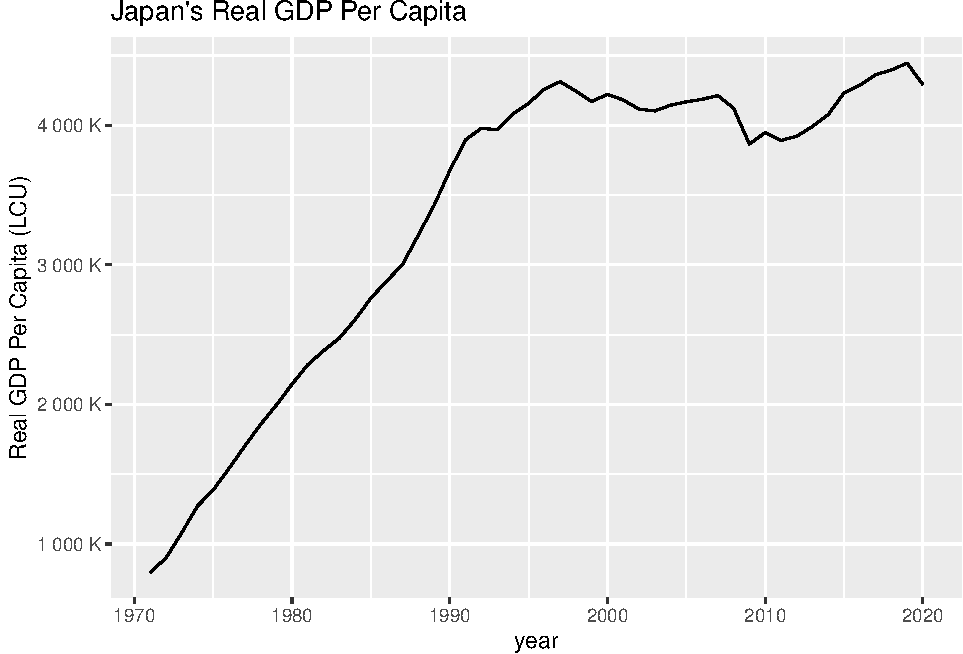
\includegraphics{rbc_report_files/figure-latex/data-1.pdf}

~~~~Next, we calculate the trend data from the above. For this, we use
the Hodrick-Prescott filtering method, specifying the smoothing
parameter \(\lambda = 100\) since we are using annual data. Beause we
are interested in the relative difference of the trend and raw data (our
focus is not on accuracy), we use log GDP data for our analysis.

\begin{Shaded}
\begin{Highlighting}[]
\CommentTok{### Compute trends}
\NormalTok{jplong.hp <-}\StringTok{ }\KeywordTok{hpfilter}\NormalTok{(}\KeywordTok{log}\NormalTok{(jplong}\OperatorTok{$}\NormalTok{gdp_percap),}\DataTypeTok{freq =} \DecValTok{100}\NormalTok{, }\DataTypeTok{type=}\StringTok{"lambda"}\NormalTok{) }\CommentTok{# hodrick-prescott filter}
\NormalTok{jplong}\OperatorTok{$}\NormalTok{trend <-}\StringTok{ }\NormalTok{jplong.hp}\OperatorTok{$}\NormalTok{trend }\CommentTok{# trend data }
\NormalTok{jplong}\OperatorTok{$}\NormalTok{cyclical <-}\StringTok{ }\NormalTok{jplong.hp}\OperatorTok{$}\NormalTok{cycle }\CommentTok{# cyclic data }
\NormalTok{jplong}\OperatorTok{$}\NormalTok{log_gdp <-}\StringTok{ }\KeywordTok{log}\NormalTok{(jplong}\OperatorTok{$}\NormalTok{gdp_percap) }\CommentTok{# log GDP }

\CommentTok{### Plot data}
\NormalTok{hpfplot <-}\StringTok{ }\KeywordTok{ggplot}\NormalTok{(jplong, }\KeywordTok{aes}\NormalTok{(}\DataTypeTok{x=}\NormalTok{year)) }\OperatorTok{+}
\StringTok{  }\KeywordTok{geom_line}\NormalTok{(}\KeywordTok{aes}\NormalTok{(}\DataTypeTok{y=}\NormalTok{log_gdp, }\DataTypeTok{colour =} \StringTok{"Log(Real GDP per Capita)"}\NormalTok{)) }\OperatorTok{+}
\StringTok{  }\KeywordTok{geom_line}\NormalTok{(}\KeywordTok{aes}\NormalTok{(}\DataTypeTok{y=}\NormalTok{trend, }\DataTypeTok{colour =} \StringTok{"Trend"}\NormalTok{)) }\OperatorTok{+}\StringTok{ }
\StringTok{  }\KeywordTok{scale_color_manual}\NormalTok{(}\StringTok{""}\NormalTok{, }
                     \DataTypeTok{breaks=}\KeywordTok{c}\NormalTok{(}\StringTok{"Log(Real GDP per Capita)"}\NormalTok{, }\StringTok{"Trend"}\NormalTok{), }
                     \DataTypeTok{values=}\KeywordTok{c}\NormalTok{(}\StringTok{"darkred"}\NormalTok{, }\StringTok{"steelblue"}\NormalTok{)) }\OperatorTok{+}\StringTok{ }
\StringTok{  }\KeywordTok{labs}\NormalTok{(}\DataTypeTok{x =} \StringTok{"year"}\NormalTok{, }\DataTypeTok{y=}\StringTok{""}\NormalTok{, }\DataTypeTok{title=}\StringTok{"Hodrick-Prescott filter of Log(GDP per capita)"}\NormalTok{) }
\NormalTok{hpfplot}
\end{Highlighting}
\end{Shaded}

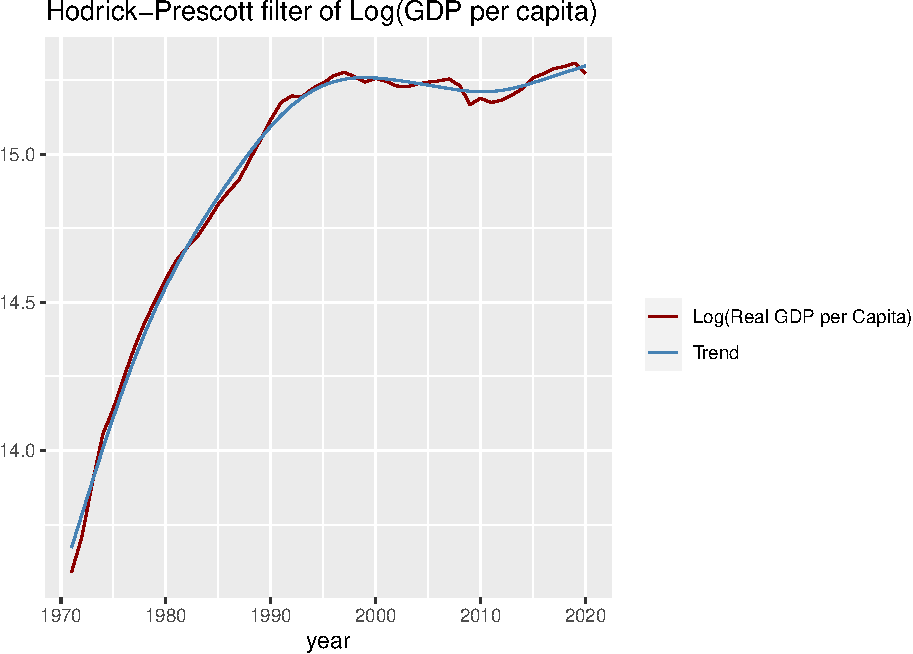
\includegraphics{rbc_report_files/figure-latex/unnamed-chunk-1-1.pdf}

~~~~Next, we find the cyclical component (business cycles) of the data.
This is computed from the difference between the raw and trend data we
have computed above. Furthermore, since we are interested in describing
the characteristics of these cycles, we also separately compute and
highlight the peaks of the cycles. The peaks can be defined as points of
the cycle which exceed in value from their adjacent points in a
neighborhood of \(m\). Here we use \(m=2\), so the peaks in the data
shown below are points whose value exceeds 2 points immediately
preceding them and 2 points immediately succeeding them.

\begin{Shaded}
\begin{Highlighting}[]
\CommentTok{### Finding Peaks }
\NormalTok{find_peaks <-}\StringTok{ }\ControlFlowTok{function}\NormalTok{ (x, }\DataTypeTok{m =} \DecValTok{2}\NormalTok{)\{}
  \CommentTok{# define peak as t: t >= [t-m, t+m]}
\NormalTok{    shape <-}\StringTok{ }\KeywordTok{diff}\NormalTok{(}\KeywordTok{sign}\NormalTok{(}\KeywordTok{diff}\NormalTok{(x, }\DataTypeTok{na.pad =} \OtherTok{FALSE}\NormalTok{)))}
\NormalTok{    pks <-}\StringTok{ }\KeywordTok{sapply}\NormalTok{(}\KeywordTok{which}\NormalTok{(shape }\OperatorTok{<}\StringTok{ }\DecValTok{0}\NormalTok{), }\DataTypeTok{FUN =} \ControlFlowTok{function}\NormalTok{(i)\{}
\NormalTok{       z <-}\StringTok{ }\NormalTok{i }\OperatorTok{-}\StringTok{ }\NormalTok{m }\OperatorTok{+}\StringTok{ }\DecValTok{1}
\NormalTok{       z <-}\StringTok{ }\KeywordTok{ifelse}\NormalTok{(z }\OperatorTok{>}\StringTok{ }\DecValTok{0}\NormalTok{, z, }\DecValTok{1}\NormalTok{)}
\NormalTok{       w <-}\StringTok{ }\NormalTok{i }\OperatorTok{+}\StringTok{ }\NormalTok{m }\OperatorTok{+}\StringTok{ }\DecValTok{1}
\NormalTok{       w <-}\StringTok{ }\KeywordTok{ifelse}\NormalTok{(w }\OperatorTok{<}\StringTok{ }\KeywordTok{length}\NormalTok{(x), w, }\KeywordTok{length}\NormalTok{(x))}
       \ControlFlowTok{if}\NormalTok{(}\KeywordTok{all}\NormalTok{(x[}\KeywordTok{c}\NormalTok{(z }\OperatorTok{:}\StringTok{ }\NormalTok{i, (i }\OperatorTok{+}\StringTok{ }\DecValTok{2}\NormalTok{) }\OperatorTok{:}\StringTok{ }\NormalTok{w)] }\OperatorTok{<=}\StringTok{ }\NormalTok{x[i }\OperatorTok{+}\StringTok{ }\DecValTok{1}\NormalTok{])) }\KeywordTok{return}\NormalTok{(i }\OperatorTok{+}\StringTok{ }\DecValTok{1}\NormalTok{) }\ControlFlowTok{else} \KeywordTok{return}\NormalTok{(}\KeywordTok{numeric}\NormalTok{(}\DecValTok{0}\NormalTok{))}
\NormalTok{    \})}
\NormalTok{     pks <-}\StringTok{ }\KeywordTok{unlist}\NormalTok{(pks)}
\NormalTok{     pks}
\NormalTok{\}}
\NormalTok{peaks <-}\StringTok{ }\KeywordTok{find_peaks}\NormalTok{(jplong}\OperatorTok{$}\NormalTok{cyclical)}
\NormalTok{year_pks <-}\StringTok{ }\NormalTok{jplong}\OperatorTok{$}\NormalTok{year[peaks]}
\NormalTok{cyclical_pks <-}\StringTok{ }\NormalTok{jplong}\OperatorTok{$}\NormalTok{cyclical[peaks]}
\NormalTok{peaksdf <-}\StringTok{ }\KeywordTok{data.frame}\NormalTok{(year_pks, cyclical_pks)}

\CommentTok{### Plotting Business Cycles}
\NormalTok{cyclicalplot <-}\StringTok{ }\KeywordTok{ggplot}\NormalTok{(jplong, }\KeywordTok{aes}\NormalTok{(}\DataTypeTok{x=}\NormalTok{year, }\DataTypeTok{y=}\NormalTok{cyclical)) }\OperatorTok{+}
\StringTok{  }\KeywordTok{geom_line}\NormalTok{() }\OperatorTok{+}\StringTok{ }
\StringTok{  }\KeywordTok{geom_point}\NormalTok{(}\DataTypeTok{data=}\NormalTok{peaksdf, }\KeywordTok{aes}\NormalTok{(}\DataTypeTok{x=}\NormalTok{year_pks, }\DataTypeTok{y=}\NormalTok{cyclical_pks), }\DataTypeTok{color=}\StringTok{"red"}\NormalTok{) }\OperatorTok{+}\StringTok{ }
\StringTok{  }\KeywordTok{labs}\NormalTok{(}\DataTypeTok{x =} \StringTok{"year"}\NormalTok{, }\DataTypeTok{y=}\StringTok{""}\NormalTok{, }\DataTypeTok{title=}\StringTok{"Japanese Business Cycles"}\NormalTok{) }\OperatorTok{+}
\StringTok{  }\KeywordTok{geom_hline}\NormalTok{(}\KeywordTok{aes}\NormalTok{(}\DataTypeTok{yintercept=}\DecValTok{0}\NormalTok{), }\DataTypeTok{color =} \StringTok{"red"}\NormalTok{)}
\NormalTok{cyclicalplot}
\end{Highlighting}
\end{Shaded}

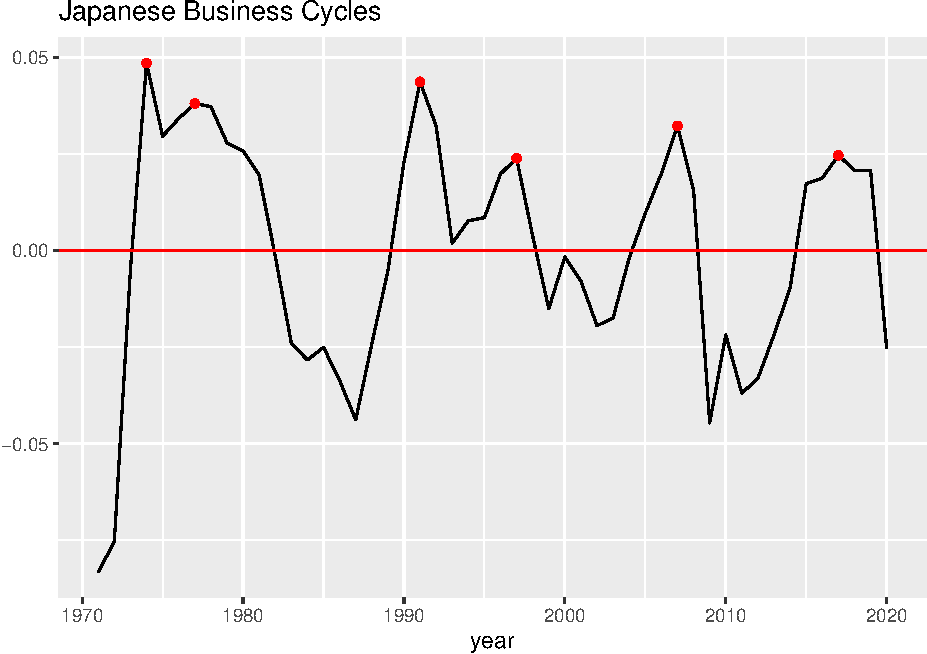
\includegraphics{rbc_report_files/figure-latex/unnamed-chunk-2-1.pdf}
From the above, we can count 9 peaks in our data. Sure enough, the
cycles seem to be occurring at regular intervals, although the high
concentration of cyclical fluctuation between 1990 and 2000 is
characteristic of Japan and the Bubble inflation it experienced during
this period as well as other shocks. The amplitude of the fluctuations
in the cycles seems to be diminishing as the years progress, but the
intervals seem pretty much consistent. Although the cycles vary quite
widely, there is no noticeable pattern to them, suggesting that the
mechanism behind their creation is stable. The mean number of years
between peaks is about 5.4 years.

\begin{Shaded}
\begin{Highlighting}[]
\KeywordTok{mean}\NormalTok{(}\KeywordTok{diff}\NormalTok{(peaksdf}\OperatorTok{$}\NormalTok{year))}
\end{Highlighting}
\end{Shaded}

\begin{verbatim}
## [1] 8.6
\end{verbatim}

\newpage

\hypertarget{building-the-model}{%
\section{Building the Model}\label{building-the-model}}

~~~~Because our purpose in this paper is to elucidate the process of
macroeconomic research in as straightforward a manner as possible, the
model we provide prioritizes simplicity over accuracy.\\
\hspace*{0.333em}\hspace*{0.333em}\hspace*{0.333em}\hspace*{0.333em}Instead
of dealing with a model with an infinitely lived agent, where
uncertainty significantly complicates the problem, we reduce our model
to dealing with a representative agent who lives for one period only.
The agent's primary concern is \(c_t\), or their consumption in that
period. However, we also assume that this person has a child who lives
in the next period, and passes on capital \(k_{t+1}\) to the child,
determined by the standard law of motion for capital (i.e., sum of
depreciated inherited capital and investment). Furthermore, every
individual in our model uses their resources to determine their
consumption and investment. Their resources are determined by the
capital they receive from their parents preceding them, and goes through
a production function which considers a stochastic shock \(z_t\) to
total factor productivity (for convenience, we separate the stochastic
shock and the TFP \(B\)). Combining all of this, we have our problem:
\[\begin{aligned}
\max \;&U(c_t, k_{t+1}) \; \;\;\; s.t. \\
&c_t + i_t = F(k_t, z_t)  \\
&k_{t+1} = (1 - \delta) k_t + i_t
\end{aligned}\]

~~~~Let us assume the form of the functions \(U()\) and \(F()\), which
are the utility function and production function respectively. Let
\(U(c_t, k_{t+1}) = \log (c_t) + A \log (k_{t+1})\) and
\(F(k_t, z_t) = Bk_t^{\frac{1}{2}} + z_t\). Note that the total factor
productivity \(B\) is constant, and we represent stochastic shocks as a
separate variable \(z_t\). However, this can still be interpreted as a
shock to total factor productivity.\\
\[\begin{aligned}
\max \;\;&\log (c_t) + A \log (k_{t+1}) \; \;\;\; s.t. \\
&c_t + i_t = Bk_t^{\frac{1}{2}} + z_t  \\
&k_{t+1} = (1 - \delta) k_t + i_t
\end{aligned}\] ~~~~Now, we can derive the solution to our model:
\[\begin{aligned}
\max \;\;\log \left(Bk^\frac{1}{2} + z_t - i_t\right) + A\log\left((1 - \delta) k_t + i_t\right)
\end{aligned}\] Taking the first order condition with respect to
\(i_t\), we have
\[-\frac{1}{B\sqrt{k_t} + z_t - i_t} + \frac{A}{(1 - \delta) k_t + i_t} = 0\]
Solving this, we get \[\begin{aligned}
i_t^* &= \frac{A[B\sqrt{k_t} + z_t] - (1-\delta)k_t}{1 + A} \\
\implies c_t^* &= \frac{B\sqrt{k_t} + z_t + (1- \delta)k_t}{1 + A}
\end{aligned}\]

~~~~Notice the following: \[\begin{aligned}
\frac{\partial}{\partial z_t}i_t^* &= \frac{A}{1 + A} \\
\implies \frac{\partial}{\partial z_t}c_t^* &= \frac{1}{1 + A}
\end{aligned}\] Assuming \(A>1\), which is reasonable, the above is in
congruence with the well known fact that investment responds more
sharply to business cycle fluctuations than does consumption.

\hypertarget{simulation}{%
\section{Simulation}\label{simulation}}

~~~~In this section, we simulate our model to observe how well it
approximates the process of real business cycle shocks. In our model,
\(A\) is roughly the ratio of consumption and capital in the steady
state. We could in theory calibrate \(A\) to fit the empirical reality
and improve upon our model, but for now we let \(A=4\). \(B\) is the
constant element of total factor productivity, and only affects the
scale of the graph for our simulation, not the shape, and thus is of
secondary importance. We let \(B = 0.3\). The depreciation rate
\(\delta = 0.025\). Now, we simulate \(c\) and \(i\) and \(gdp = c + i\)
in our economy by specifying the initial level of capital \(k_0 = 3.7\).
Furthermore, we examine the case for two distributions of the random
shock \(z\), \(z\sim Unif[0,1]\) and \(z \sim N(0, 0.17)\). The results
are as follows: 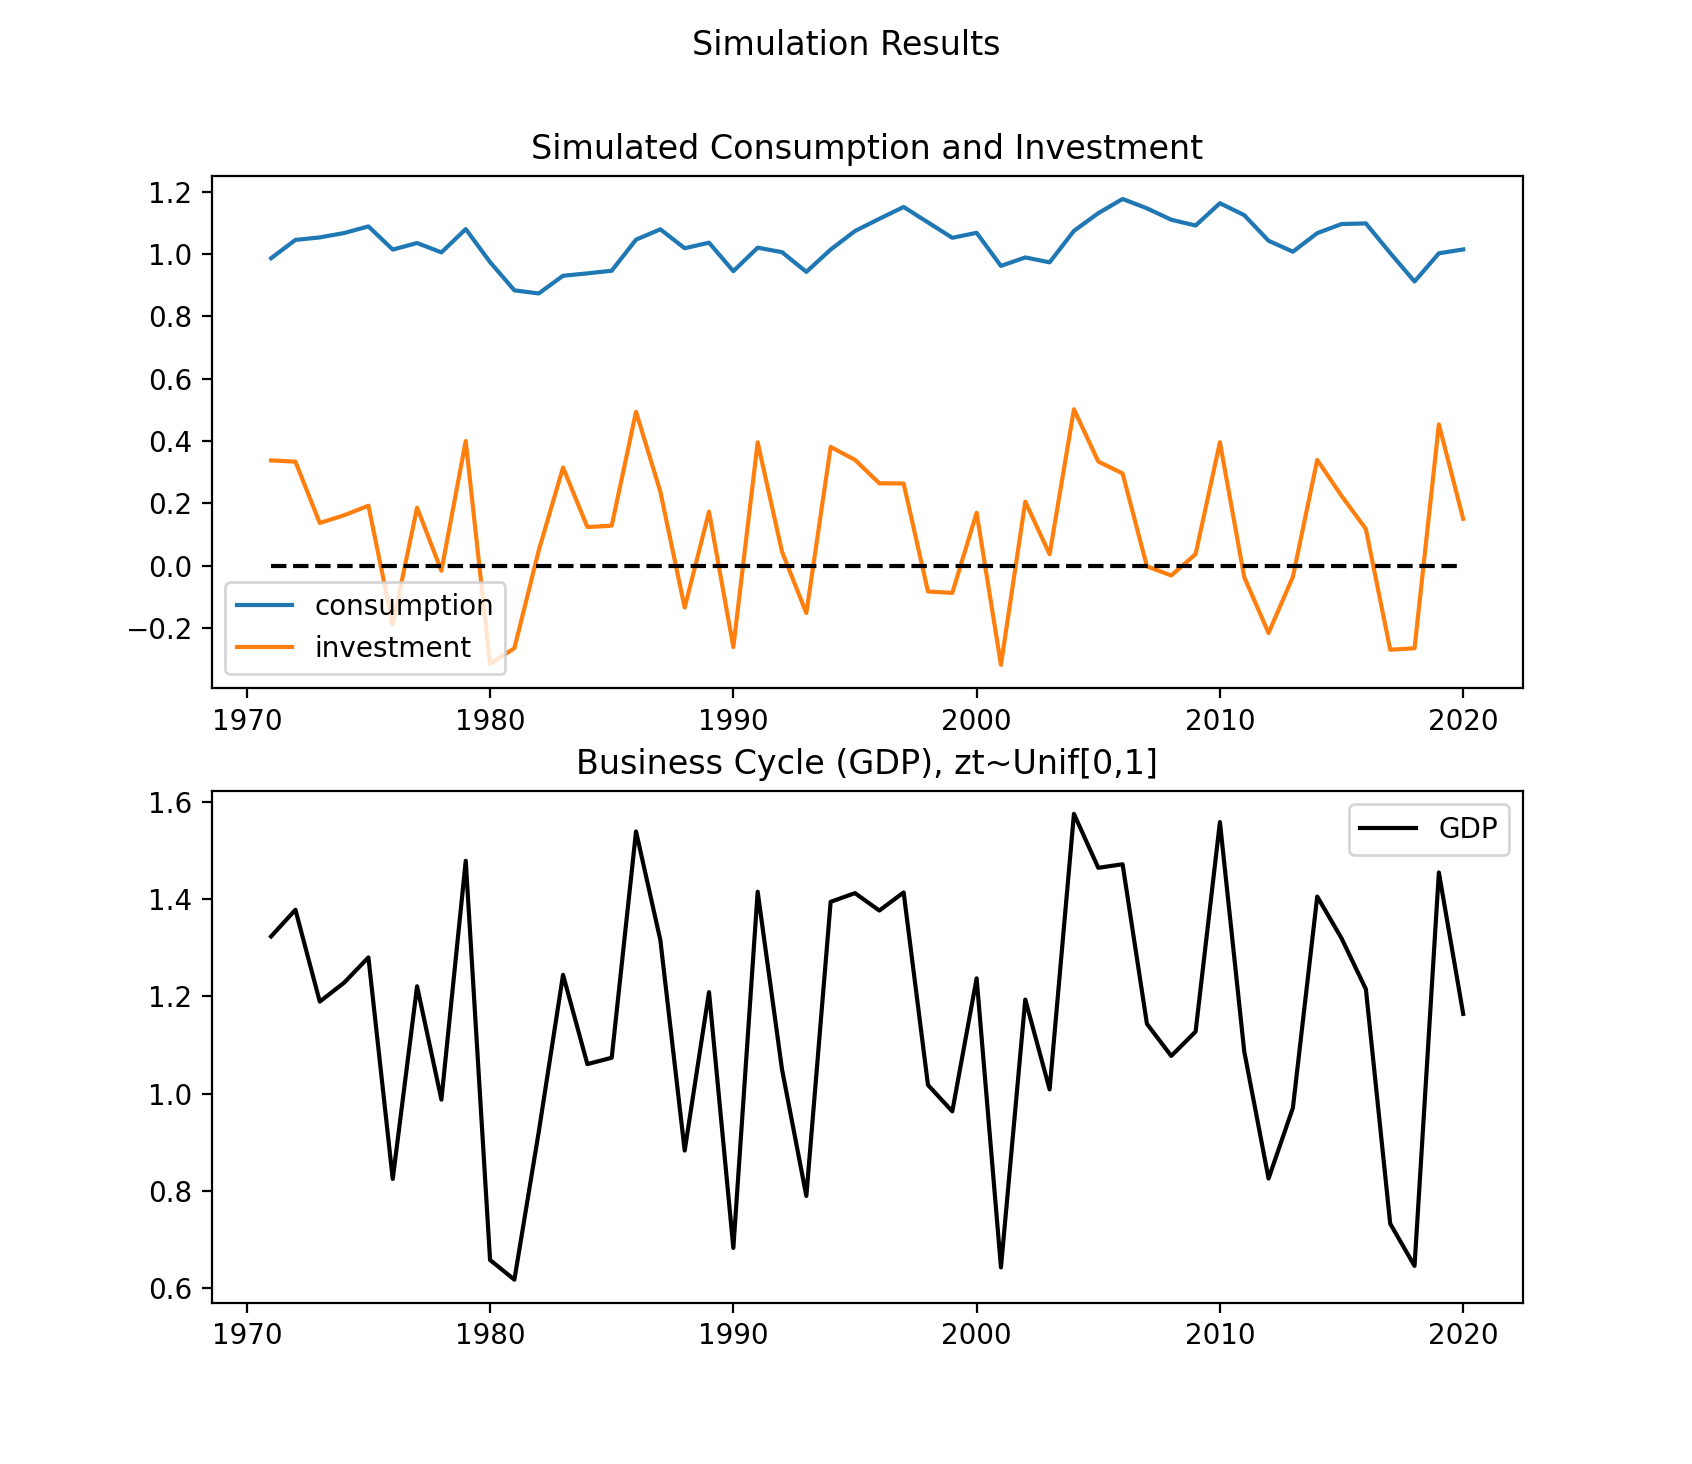
\includegraphics{data/sim_uniform_shock.png}\\
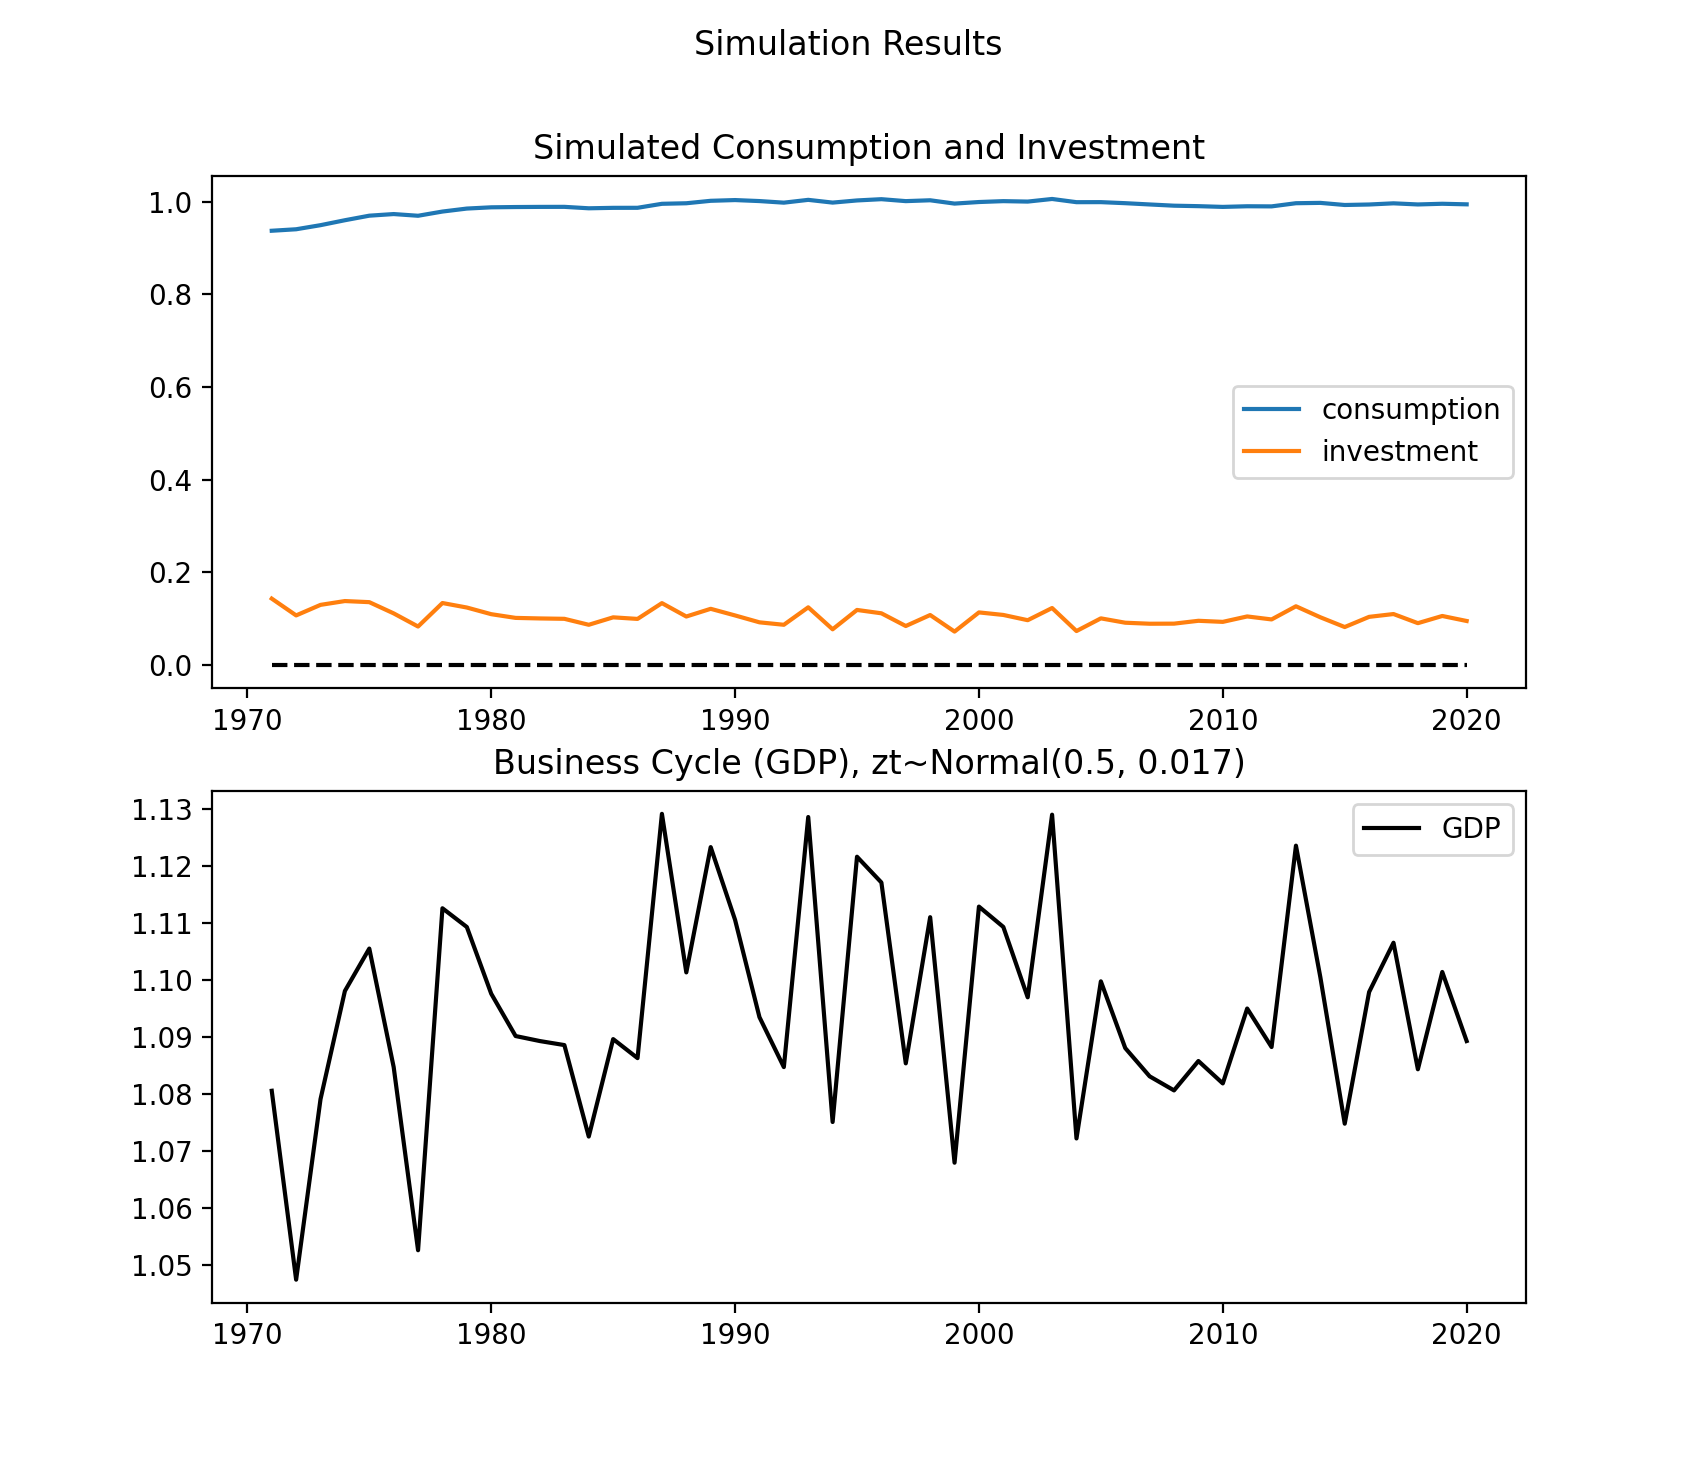
\includegraphics{data/sim_normal_shock.png}

~~~~The simulation results show us that our model indeed produces
cyclical fluctuations in GDP data, and hints towards the workings of
real business cycles in real life. While consumption in both cases is
relatively constant across time, investment is heavily influenced by the
stochastic shocks of each period, creating the source for the business
cycle fluctuations. We can observe that with the normal distribution,
the amplitude of the cycles are much smaller than those of the uniform
distribution. The normal distribution does a better job of capturing the
nature of actual stochastic shocks to productivity in the sense that
high magnitude shocks do not occur so frequently. Both graphs, when
compared to the original graph charting Japanese real business cycles,
do differ quite heavily in characteristics. Perhaps greater care in
selecting parameters to the model, which is known as ``model
calibration'', could somewhat improve its accuracy. Indeed, many
macroeconomic studies rely on calibration to assess the accuracy of and
develop on models.

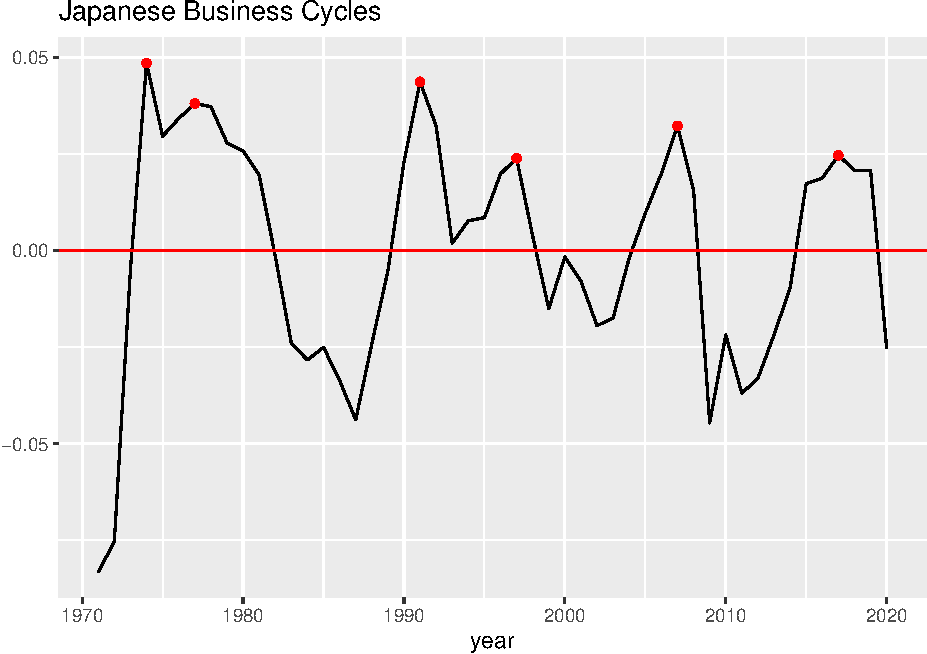
\includegraphics[width=0.5\linewidth]{rbc_report_files/figure-latex/unnamed-chunk-5-1}
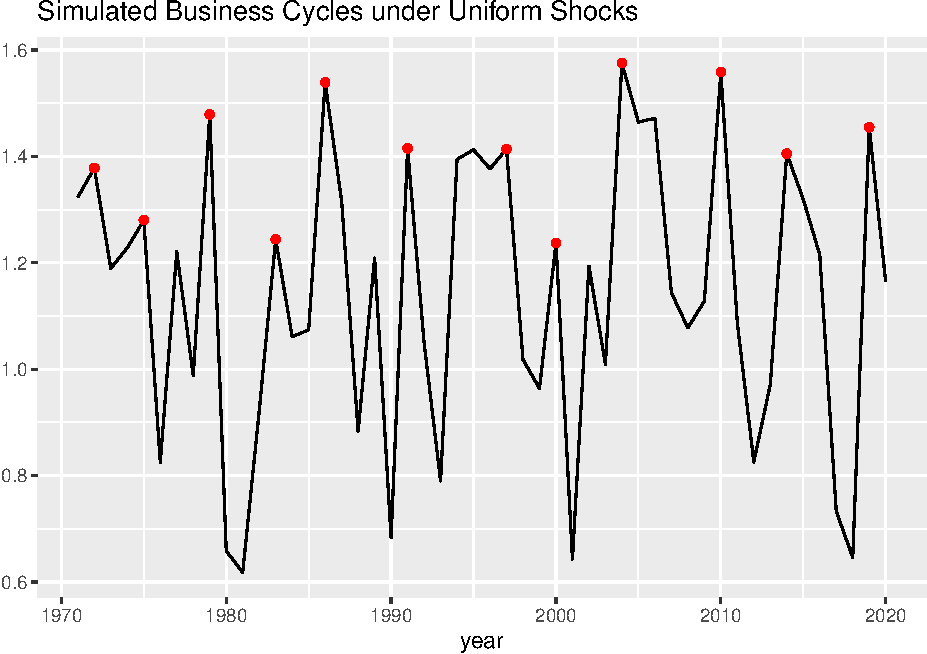
\includegraphics[width=0.5\linewidth]{rbc_report_files/figure-latex/unnamed-chunk-5-2}

~~~~When comparing the simulation results for uniform shocks with
Japanese business cycles, we immediately notice that there are far more
cycles in the simulation than there are in the empirical data. This
suggests that are model is overestimating the variance of the random
shocks to productivity. The variation in amplitude of cycles, however,
is similar, although there is no sign of the amplitude decreasing over
time in our model. Both graphs have high variation in amplitude.
However, there is no observable trend to the position of the peaks of
the simulated business cycles as there seems to be in the Japanese
business cycles. I assume this is due to real life stochastic shocks
being dependent on preceding shocks, and not independent of them. In our
simulation, all shocks were modeled as independent, making it difficult
for such a pattern to emerge. Finally, the mean distance between peaks
for our simulated model is significantly less than the mean distance
between peaks for the empirical data.

\begin{Shaded}
\begin{Highlighting}[]
\KeywordTok{mean}\NormalTok{(}\KeywordTok{diff}\NormalTok{(simpeaksdf}\OperatorTok{$}\NormalTok{year))}
\end{Highlighting}
\end{Shaded}

\begin{verbatim}
## [1] 4.272727
\end{verbatim}

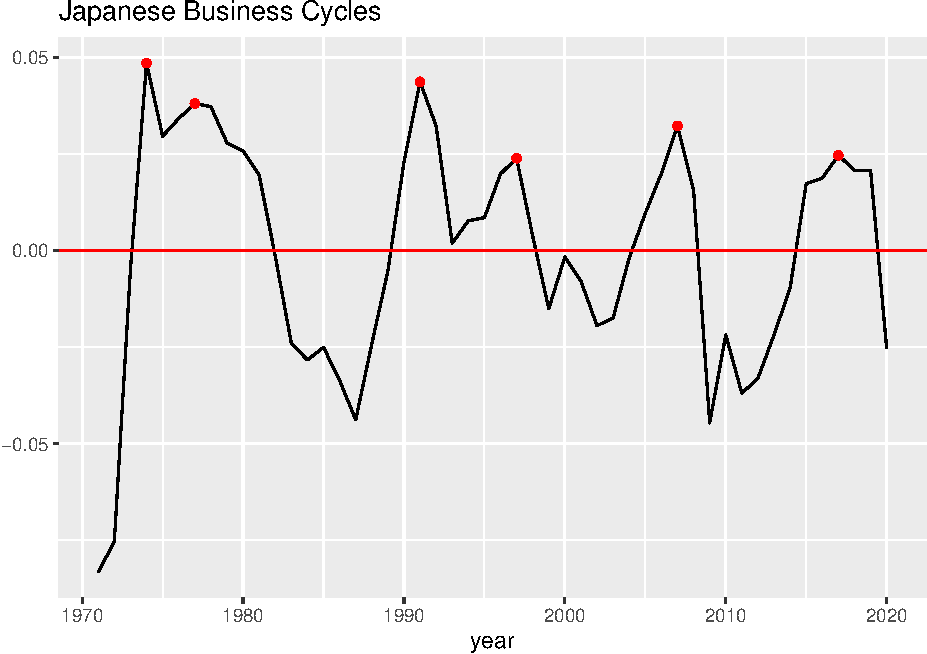
\includegraphics[width=0.5\linewidth]{rbc_report_files/figure-latex/unnamed-chunk-8-1}
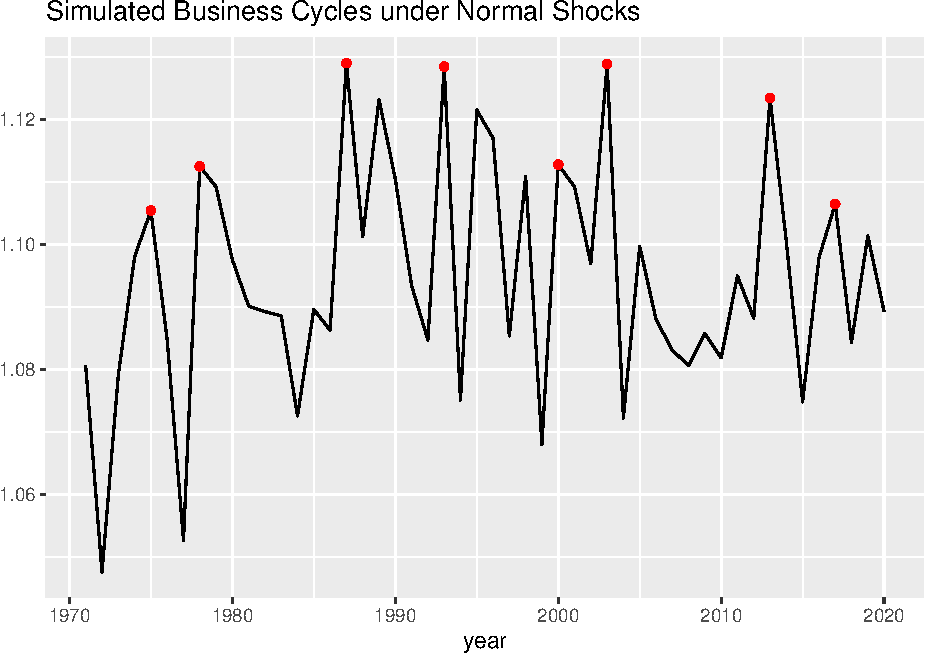
\includegraphics[width=0.5\linewidth]{rbc_report_files/figure-latex/unnamed-chunk-8-2}

~~~~The simulation under normal shocks is somewhat better at
approximating real life business cycles than the simulation under
uniform shocks, although it is still not much of an improvement. In the
model under normal shocks, we have 8 peaks, just two more than the
empirical data. Furthermore, the position of the peaks seems to be
closer together than the uniform data, making it more similar to the
real Japanese business cycles. However, the limitations we discussed
earlier are also applicable here. The shape of the cycles do not seem to
be strongly related to each other, and thus is a poor reflection of the
shape of the Japanese business cycles. The amplitude of the cycles does
not have any clear pattern either. The mean between the peaks is 6
years, while the Japanese business cycles generally had intervals of
around 8 years.

\begin{Shaded}
\begin{Highlighting}[]
\KeywordTok{mean}\NormalTok{(}\KeywordTok{diff}\NormalTok{(simpeaksdf}\OperatorTok{$}\NormalTok{year))}
\end{Highlighting}
\end{Shaded}

\begin{verbatim}
## [1] 6
\end{verbatim}

~~~~Our model did not have a government nor did it have a central bank,
and the lack of such a stabilizing entity may also be one of the sources
of discrepancies between it and the real world.

\hypertarget{conclusion}{%
\section{Conclusion}\label{conclusion}}

~~~~All in all, our model showed us that it is possible to model
cyclical fluctuations in output with the neoclassical growth model by
introducing stochastic shocks. In real business cycle analysis,
researchers aim to further the understanding of business cycles by
formulating such fully specified stochastic models and testing them via
``calibration''. Although the accuracy of our model could be heavily
improved on, at the very least it shows the creativity and
appropriateness of this approach to studying business cycles.

\hypertarget{references}{%
\section{References}\label{references}}

\setlength{\parindent}{-0.2in}
\setlength{\leftskip}{0.2in}
\setlength{\parskip}{8pt}

\noindent

Plosser, Charles. 1989. ``Understanding Real Business Cycles''. Journal
of Economic Perspectives 3(3): 51-78.

The World Bank, World Development Indicators (2012). Real GDP per capita
(LCU). Retrieved from
\url{https://data.worldbank.org/indicator/NY.GDP.PCAP.CN?locations=JP}

\end{document}
